\documentclass[12pt]{book}
\usepackage[utf8]{inputenc}
\usepackage{a4wide}
\usepackage{amsmath}
\usepackage{hyperref}
\usepackage{times}
\usepackage{graphicx}

\begin{document}

\chapter{Collaborative Cheminformatics Applications}

\section{Background}

Cheminformatics deals with the aggregation, handling, processing, and
analysis of chemical data. The nature of the chemical data is in principle
not important, but the history of the field and its separation from
quantum chemistry fields, bias the field towards small organic molecules.
The patterns in collaborative applications are, however, independent from
the exact nature of the data. Instead, we will focus in this chapter
on another dimension to discuss the aspects of collaborative
cheminformatics applications: code development, knowledge handling
and data exchange, and collaborative computation.

The first section will focus on methods involved in the collaborative
development of cheminformatics software, and discuss the tools modern
scientists have to perform this task. The next section will describe
recent changes in which we handle chemical data and knowledge, and
in particular how the Internet is changing how communities crate new
knowledge bases. The third section will focus on the aspects of
collaborative computing in cheminformatics.

A fourth section describes social aspects of collaborative projects,
and in particular how collaboration is managed in projects with
only loosly defined roles of the various partners.

\section{Collaborative Cheminformatics Code Development}

Collaborative code development is a common approach for large software vendors.
For scientific software, however, it is more uncommon: new software is typically
started as a PhD or M.Sc. project, with a single developer. There are, though,
two areas where collaborative code development in cheminformatics flourishes:
one situation is where a piece of software has become large and successful,
and multiple people have interest in contributing to the project; the second
situation is where the project is fairly small, and no single developer can
or wants to lead the project, as the topic is not core business.

An example of the latter situation is the JChemPaint project. There are existing
similar projects, making continued development out of scope of cheminformatics
research. However, Steinbeck et al. showing in 1998 that a collaborative project
can lead to an eco system where such software can still be
developed~\cite{Krause2000}.

Central to collaborative code development is sharing source code. Particularly,
it is pipelining how patches are shared and applied. While some cheminformatics
projects still share source code as source distributions, the adoption of
source code repositories as the golden standard. There are various 
open source repository technologies around, including Concurrent Versions System (CVS),
Subversion (SVN), Mercurial, Bazaar, and Git. CVS is the oldest and mostly replaced
by the newer technologies. Subversion is still abundant, but increasingly
replaced by the last three technologies. The reason for this is that
those three are distributed technologies, allowing server redundancy.

Moreover, because of the distributed nature of Mercurial, Bazaar, and Git,
branching and merges of branches is often easier. However, the increased
functionality also introduces further complexity, which is particularly
the case for Git, causing an increased learning curve.

As these tools are Open Source, anyone is able to set up a local server, but
Open Source projects can take advantage of service providers that host
free and public code repositories. Table~\ref{tab:cvsProviders}
provides an overview of various larger service providers, but there
are many alternatives.

\begin{table}
\caption{Overview of code sharing technologies and service providers
that provide free hosting:
GitHub: \url{https://github.com/},
Gitorious: \url{https://gitorious.org/},
Google Code: \url{http://code.google.com/},
LaunchPad: \url{https://launchpad.net/},
SourceForge: \url{https://sf.net/}.
}
\label{tab:cvsProviders}
\vspace{0.1cm}
\begin{center}
\begin{tabular}{c|c}
\textbf{Technology} & \textbf{Provider(s)} \\ 
\hline Concurrent Versions System &  SourceForge \\ 
\hline Subversion & SourceForge, Google Code \\ 
\hline Mercurial & Google Code \\ 
\hline Bazaar & LaunchPad \\ 
\hline Git & GitHub, Gitorious, SourceForge \\ 
\end{tabular} 
\end{center}
\end{table}

\subsection{Licensing}

Another aspect that makes collaboration easier, is to use an
Open Source license. Such a license ensures that potential
contributors know that whatever work they invest in the source
code is not lost: it will always be available to that
contributor under those license terms.
There are various Open Source licenses available, with
different characteristics. A discussion on differences and
details is well beyond the scope of this chapter, however.
They reader is kindly invited to read the book
Open Source Licensing by Lawrence Rosen~\cite{Rosen2004}.
Popular Open Source licenses include the GPL
licenses, and the MIT and BSD licenses. A full overview of Open
Source licenses is available from the Open Source Initiative:
\url{http://www.opensource.org/licenses}.

\subsection{Peer review}

Another aspect of collaborative development is that one can
take advantage of peer review. While the role of peer review
in scientific publishing is well recognized, it is hardly
applied to scientific programming. Nevertheless, the
advantages are clearly recognized, such as written up
in the famous writing \textit{The Cathedral and the Bazaar}~\cite{Raymond2001}:

\begin{quotation}
It's one thing to observe in the large that the bazaar style
greatly accelerates debugging and code evolution. It's
another to understand exactly how and why it does so at the
micro-level of day-to-day developer and tester behavior.
\end{quotation}

The section then details on why the Bazaar model, with many
people looking at the code actually works. Now, interestingly,
this is where it may not apply to cheminformatics, where
the number of potential people looking at the code is
relatively low. Moreover, developers from competing projects
may have additional reasons not to review work from other
projects, further reducing the number of reviewers.

It should be noted that this problem is general to science,
and that peer review of publications too typically requires
a more formal approach. Code development has the advantage
that static source code checkers are available that can
detect common problems, such as PMD (\url{http://pmd.sf.net/}).
These tools check, for example, for unused variables, dead
code, etc, often highlighting sources of problems.

Manual peer code review is increasingly simplified by new
tools. For example, GitHub provides the functionality to
comment on changes~\cite{Chemblaics201005CodeReview},
increasing the communication between developers and the
social pressure to write better source code.
Figure~\ref{fig:githubCodereview} show an example comment
made via the GitHub website.

\begin{figure}
\begin{center}
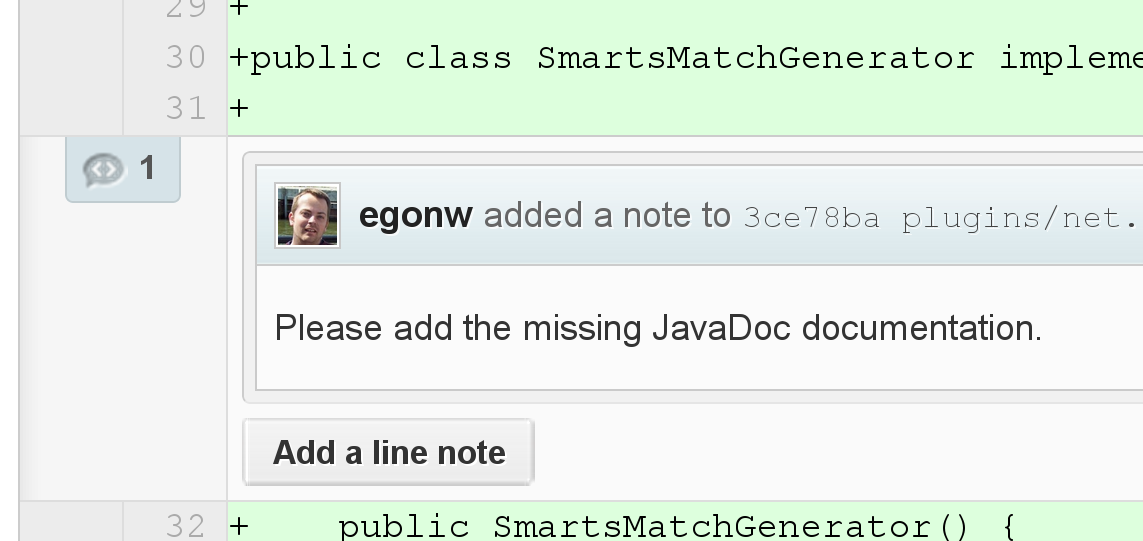
\includegraphics[width=0.8\textwidth]{graphics/codeReview8.png}
\end{center}
\caption{Screenshot of the GitHub webpage providing code
review functionality. The comments shows a reviewer question
regarding a parameter description missing in the JavaDoc
(see \url{http://github.com/egonw/bioclipse.cheminformatics/commit/3ce78ba}).}
\label{fig:githubCodereview}
\end{figure}

\section{Collaborative Cheminformatics Knowledge Base Building}

Open Data ...

The Blue Obelisk Data Repository is a collaborative project by a number
of cheminformatics tools, including Kalzium (of the KDE desktop), the
Chemistry Development Kit, ...

\begin{figure}
\begin{center}
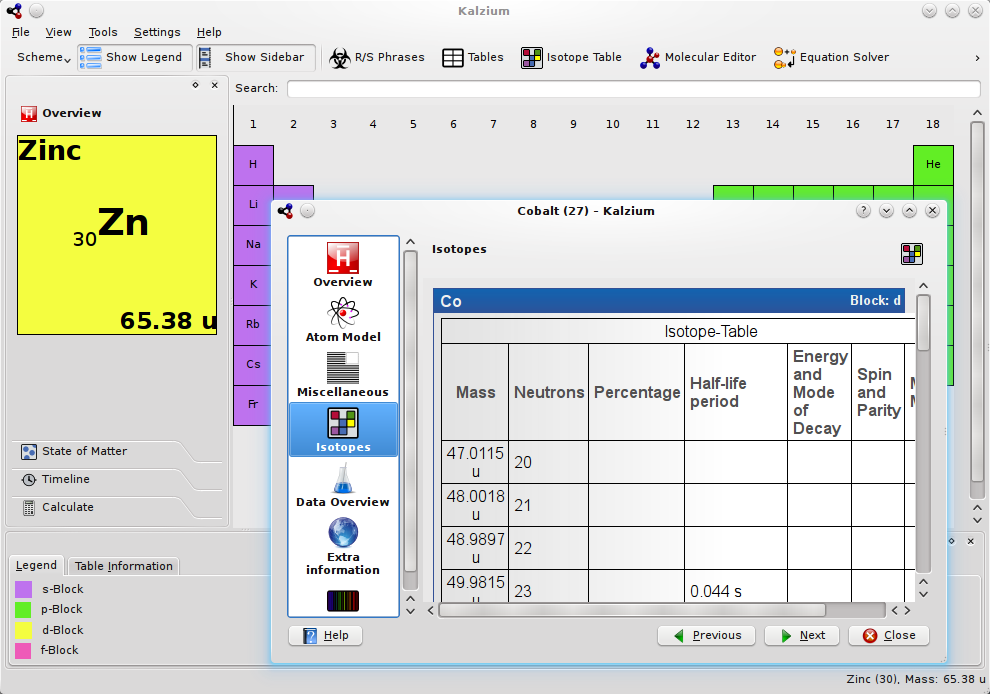
\includegraphics[width=0.8\textwidth]{graphics/kalzium.png}
\end{center}
\caption{Screenshot of the Kalzium, part of the KDE Software
Compilation (\url{http://kde.org/}), showing information on the
isotopes of cobalt using the Blue Obelisk Data Repository.}
\label{fig:kalzium}
\end{figure}

Social sites to share Open Data include the
NMRShiftDB~\cite{Steinbeck2004} (GNU FDL license),
ChemPedia (\url{http://chempedia.org/substances}, CC0 license)...

% TODO: perhaps move these resources into a table

\subsection{Linking Knowledge Bases}

Key to collaboration is also the sharing of knowledge. A prominent role here
plays the linking of various databases, which allows integration of them.

Resource Description Framework ... HCLS, Bio2RDF, Chem2Bio2RDF, ...

Userscripts present an approach to linking resources with a very low
barrier to entry. The idea of a Userscript was first made available by
the Greasemonkey Mozilla extension and later by Ubiquity Mozilla
extension. A userscript was simply a small Javascript program that
runs on the client browser and can modify a given web page before it
is displayed to the viewer. In other words, given permission to do so,
a userscript can completely rewrite a webpage in any way it sees
fit. This opens up exciting possibilities in annotating web content
and linking web content to arbitrary data sources. A variety of
userscripts for cheminformatics have been described by Willighgen et
al~\cite{Willighagen2007b}. For example, when viewing a web page describing
chemistry, a userscript can be written to take the text and run it
through a chemical entity recognition tool (such as OSCAR [REF]) and
then highight terms that were recognized. Such a script can be further
enhanced by not only highlighting recognized terms, but inserting
hyperlinks to chemical databases such as Pubchem or
Chemspider. Another application described by Willighagen et al, was to
display 3D structures of molecules when browsing Pubchem web pages. In
the past, Pubchem did not provide 3D structure information. On the
other hand, Indiana University had generated a single low energy
conformer for 99\% of Pubchem and stored them in a database. A
usercript was implemented that when run on a Pubchem compound page,
would identify the compound ID and retrieve the corresponding 3D
structure (if available) from the Indiana University database and then
display it in a Jmol window. Key to the functionality of many
cheminformatics userscripts is the use of freely accessible
cheminformatics web services (Section \ref{ref:ws}) and databases.

\section{Collaborative Computing}

The development of infrastructure and tools to link knowledge bases is
a fundamental requirement for efficient colaborations. The previous
seections have highlighted a variety of efforts in these areas. While
it is true that collaborative efforts (in any field) are primarily a
function of social interactions, it is important to remember that
collaborations need not be directly between individuals. Rather, they
can also be mediated by software. From this point of view, there have
been a number of developments in the last few years that allow
individuals, unrelated to each other in terms of formal collaborative
aggreements, to interact with each others' resources. But such
interactions do not necessarily have to involve remote
resources. Instead, a collaboration could also be in the form of
shared specifications.That is, individuals could collaborate on the
specification of a process or program, which would then be run locally
using each collaborators own resources. Finally, to achieve these
types of collaborative efforts, technologies to support these are
necessary; many of these are well established such as mailing lists
and chat systems, whereas a number are more recent such as service
registries. The following subsections discuss these facets of
collaborative computing in more detail.

\subsection{Shared Computing Services}
\label{ref:ws}
Distributed computing has gone through many phases starting with
Remote Procedure Calls (RPC) in the 1970a and 1980s to CORBA in the
1990s. More recently, distributed computing in the form of web
services have become a mechanism by which different groups expose both
methods (analogous to remote function calls that are the hallmark of
RPC and CORBA) as well as data. In this sense, we consider web
services to be a generalization, allowing one to provide access both
data (such as databases) and algorithms.

There are many protocols by which web services such as SOAP and
XMPP~\cite{Wagener2009}. Most web service protocols are designed to
work with multiple types of transport layers (HTTP, UDP, etc) but the
majority of web service protocols currently in use work over
HTTP. This approach results in significant;y easier deploy of services
and access to them, since HTTP is ubiquitous throughout the
Internet. For a more detailed review of web service technologies the
reader is referred to XXX and YYY.

In this section we provide a brief overview of cheminformatics web
services and some use cases highlighting the collaborative potential
of such web services.

Indiana University has developed a number of cheminformatics web
services [REF] that provide access to core cheminformatics methods
(fingerprints, 2D depiction and various molecular descriptors),
statistical techniques (using R [REF] as the backend) and chemical
database access methods. Most of these services are implemented in
Java using the Chemistry Development Kit [REF] and SOAP as the
underlying protocol. A detailed description of these services can be
found in Dong et al~\cite{Dong2007Web}. The services have been used in
a variety of scenarios. For example, the fingerprint and statistical
model services were employed by Indiana University to develop
models to predict the activity of user supplied compounds against the
NCI60 cancer cell lines. Interestingly, the final predictive model was
itself, converted to a web service and thus accessible by any SOAP client,
remote or local. Note that while the model service was also located at
Indiana University, it could easily make use of fingerprint services
located at other sites, anywhere across the world.

Recently, these web services have been forked and reimplemented as
REST based services. While SOAP services can be ``hidden'' behind a
REST interface, the reimplementation avoids the extra complexity
imposed by SOAP, by directly exposing the functionality via the REST
interface. These services can be found at
\href{http://rguha.net/rest}{http://rguha.net/rest}. Curently, the
services are hosted at multiple locations include Drexel University,
USA and Uppsala University, Sweden and are utilized by a number of
independent applications. An example is the use of these services to
enhance an Open Notebook Science (ONS) project. The ONS Solubility
Challenge is an ongoing project in which a number of research groups
have experimentally determined the solubility of a variety of solutes
in a variety of solvents. All the data generated as part of this
project is publicaly hosted on a GoogleDocs spreadsheet and outsiders
are encouraged to explore and mine the data, with the hope that their
results will be also be made Open. At the time of writing the project
has seen contributions from a number of people, including chemists,
mathematicians and programmers. As the project has grown, the number
of measurements now numbers in the hundreds. The spreadsheet contains
alphanumeric identifiers for solutes and solvents along with SMILES
representations and solubility data. In a number of cases, external
references are also included. While the use of Google Spreadsheets is
a very simple way to share data, the nature of the data makes it
unweildy to explore. In general, while numeric solubility data is
useful it is more appropriate to explore it from a chemical point of
view - that is, in terms of structures and substructures.

As a result, a simple web page interface
(\href{http://toposome.chemistry.drexel.edu/~rguha/jcsol/sol.html}{http://toposome.chemistry.drexel.edu/~rguha/jcsol/sol.html})
was developed that extract data from the Google spreadsheet via the
Google-provided Data API and presented the data or filtered subsets of
the data (based on solute or solvent identifiers, substructures or
solubility ranges). The key feature of this application is the
incorporation of chemical intelligence, by making use of
cheminformatics web services hosted at Uppsala University. By making
use of these services, the SMILES strings stored in the spreadsheet
could be filtered by the presence or absence of substructures
(specified via SMARTS). In addition, the services were also employed
to provide 2D structure depictions of the results matching satisfying
the query. From a colaborative point of view, this application is
interesting as the developer had no role in the gathering of the
solubility data and did not create the online spreadsheet. Instead,
the application made use of public data API's provided by Google and
public web services hosted at another, remote location to extract and
present data that satisfied the requirements of another, external
group (i.e., the experimentalists making the measurements).

A related application (\href{http://old.oru.edu/cccda/sl/descriptorspace/ds.php}{http://old.oru.edu/cccda/sl/descriptorspace/ds.php}) 
was developed by another researcher to
explore the chemical space (via descriptor calculations followed by
principal components analysis). This application also made use of the
cheminformatics services hosted at Drexel University as well as
visualization services provided by Google, allowing users to generate
principal component plots of the solubility data, thereby
understanding the extent of the chemical space occupied by the current
set of chemical.

These applications highlight the fact that distributed software
resources were key in allowing multiple, unrelated parties to
collaborate on a publically available dataset. While this type of
collaboration could certainly be achieved using traditional software
resources (i.e., locally installed libraries and programs), the
presence of freely accessible web services (for both cheminformatics
as well as data and visualization) allows \emph{arbitrary} individuals
or groups to develop novel applications that were not considered by
the original researchers. Furthermore, the free and distributed nature
of the resources allows such developers free themselves of software
installation and management and onerous licensing conditions.


\subsection{Sharing Computation Specifications}

A simple example of a ``computation specification'' is the source code
of a program or even and input file for a program. In both cases, the
document fully specifies what is required to run a program to achieve
a desired result. Clearly there have been many mechanisms to share
such specifications. However, with a few exceptions these sharing
mechanisms tend to simply collect source code, for example, in a
central repository and let users access it from there. Usually, there
is no meta data attached or associated with the source code and thus
exploring related cases is difficult.

Recently, there has been significant amounts of efforts devoted to the
development of ``workflow'' or ``pipeline'' tools for chem- and
bioinformatics. These tools encapsulate core cheminformatics tasks
such as reading in SMILES, evaluating descriptors and so on in simple
graphical elements (usually boxes and connectors). A user can then
arrange sequences of such elements to perform a task. The GUI approach
coupled with the fact that in most cases, such workflow tools require
no programming knowledge make such tools very attractive to
experimentalists and other users with limited programming
experience. A number of such tools are available including Pipeline
Pilot, KNIME and Taverna.

A recent development around workflow tools is the sharing of workflow
specifications (or ``programs''), exemplified by the MyExperiment
website~\cite{Goble2010} which allows sharing of scientific workflow
of various formats, including Taverna (see Figure~\ref{fig:myexperiment})
and Bioclipse.

\begin{figure}
\begin{center}
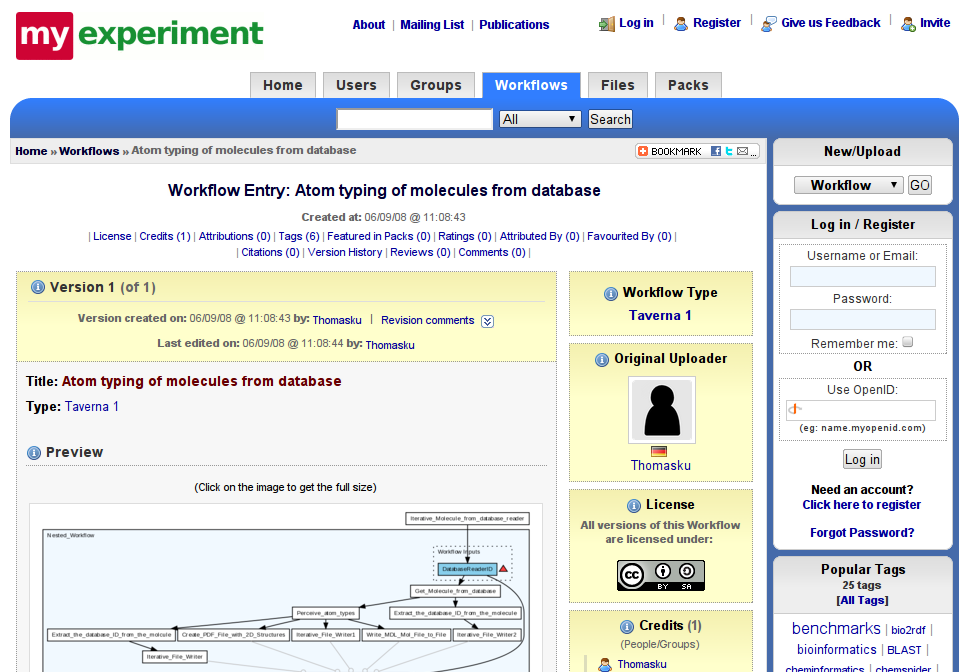
\includegraphics[width=0.8\textwidth]{graphics/myexperiment.png}
\end{center}
\caption{Screenshot of the MyExperiment.org web page for a
Taverna workflow (\url{http://www.myexperiment.org/workflows/389.html}).}
\label{fig:myexperiment}
\end{figure}

\subsection{Collaboration Tools}

Taverna~\cite{Oinn2004} ... CDK-Taverna~\cite{Kuhn2010} ...

Bioclipse~\cite{Spjuth2009,Spjuth2007}...

\section{Managing Collaborative Projects in Cheminformatics}

We have provided a brief overview of various technologies that enable
and enhance collaborative projects in the field of
cheminformatics. Yet, one aspect still remains. While tools are
available to share source code and experimental data, how are such
collaborative projects managed? When the collaboration is between two
individuals, project management is not a significant problem. It
becomes much more problematic when the number of collaborators grows
larger.

The first aspect is communication between members of the
collaboration. A number of mechanisms are available including mailing
lists and online messaging systems. Both these methods have a long
history and mailing lists are a useful way to broadcast messages to
all members of a group. This has its downside as well, as many members
may not desire such broadcasted messages. Furthermore, email is
relatively inefficient at handling multiple conversations, though
threading [REF] does alleviate this. Modern email systems such as
Google Mail have provided a number of enhancements to improve the
handling of multiple conversations in a mailing list. 

One important aspect of mailing lists is that they are not real time
or interactive. On the other hand, messaging systems such as Internet
Relay Chat (IRC) or instant messengers (Yahoo Chat, AOL, etc.) offer
real time interactivity between participants. These systems allow for
direct interactions between multiple members and are extremely useful
for on-the-fly problem solving and discussions. Of course, since these
technologies are text based, it can be slower than phone or video
conferencing. But on the otherhand, these systems are very light on
resources and efficient on slow Internet connections.

More recently, weblogs or blogs, have become a useful mode of
communication. This approach allows a degree of interactivity between
the producer of the blog and readers, but is primarily a vehicle for
an individual or group to provide updates. Of course, by allowing
multiple people to post on the blog, it can be a useful way for a
collaborative group to provide updates and information on the
project. Blogs are also useful from the consumers point of view since
they are a \emph{pull} technology. That is, the consumer (i.e.,
reader) will usually read the blog via an RSS reader and thus rather
than receive updates from the blog, will read new posts when desired.

The technologies discussed so far have focused on communication
between members of a collaboration and other interested parties. But
another vital aspect of colaborative projects is the development of
documentation - ranging from API documentation to tutorials and policy
documents. While one could exchange documents via email, one very
quickly runs into the problem of keeping everybody's edits
synchronized. Collaborative document editing systems have recently
been developed that directly address this problem. One example is
Google Docs, which is an online resource that allows one to create
documents, spreadsheets and presentations and then share them between
other users. Each authorized user can edit the document and more
importantly, multiple users can simultaneously work on these
documents. The service automatially tracks the edits by each users and
provides an intuitive view of the document history, allowing one to
view the edits made by each user. The documents can be exported to a
variety of common formats, allowing one to introduce such documents
into the traditional workflow.

Google Docs is a useful solution to the problem of collaborative
editing of traditional documents. Wikis provide another approach, that
is more free-form. The fundamental idea of a wiki is that it is a
colection of pages, linked via hyperlinks and that authorized users
can edit, add to or delete these pages arbitrarily. Most wikis will
also keep a history of the edits made to each page, allowing one to
track who did what. In contrast to something like Google Docs, wikis
are much more free form (indeed, they are fundamentally just web
pages). In addition, it is posible to add arbitrary files to a wiki,
which allows one to record and track the entire state of a project
over time (cf. the Open Notebook Science Solubility Challenge on
Wikispaces [URL]). While wikis ae useful they are not necessarily the
best solution for all cases. For example, in software development
projects, keeping an associated wiki up to date with the state of the
project can be tedious, especially if the development is very
rapid. While the wiki might be useful for material such as tutorials
and so on, it is rarely a good solution for API documentation. Many
would argue that even usage information should be a part of the API
documentation and should be written inline with the code. Such inline
documentation can easily be extracted and formatted using tools such
as Doxygen or Sphinx and \emph{linked to} from the wiki. This last
point highlights one advantage of a wiki type of system - it is a very
easy way to aggregate resources via linking rather than include them
directly in the wiki itself. This leads to significantly lower efforts
in maintaining the wiki.

In addition to these systems, tools that have traditionally been
focused on software development can be usefully applied to other
scenarios. A good example is the use of a bug tracking systems to keep
track of feature requests or new ideas. These systems allow one to
keep a list of these issues and possibly assign them to one or more
people for followup.

It should be noted that the software systems to support the ideas
described here can be obtained in a variety of forms. Each component
described here can be obtained individually, require the collaboration
to set them up whereas more comprehensive solutions also exist that
couple wiki's, feature tracking systems and collaborative editing
systems in a single package. In addition, one has a choice of Open
Source or commercial solutions to choose from.

We have dicussed a variety of technologies that facilitate
collaborative project management. But a vital component of this is the
managment of people within such projects. There are many approaches to
this ranging from committees to dictatorships (benevolent or
otherwise). In this chapter we do not discuss the merits or demerits
of any given approach, save to say that efficient personnel management
is vital to the successful completion of a collaborative project.

\section{Conclusion}

\bibliographystyle{unsrt}
\bibliography{chapter}

\end{document}

